\documentclass{ntuthesis}

\usepackage{times}
\usepackage{verbatim}
\usepackage{color}
\usepackage{url}
\usepackage{graphicx}
\usepackage{array}
\usepackage{wallpaper}
\usepackage{hyperref}
\usepackage[printwatermark]{xwatermark}
\usepackage{graphicx}
\usepackage{pdfpages}
\usepackage{indentfirst}
\usepackage{enumerate}
\usepackage{eso-pic}
\usepackage{float} %设置图片浮动位置的宏包
\usepackage{subfigure} %插入多图时用子图显示的宏包
\usepackage{listings}%程式碼高亮
\usepackage{xcolor}
\usepackage{booktabs} %需要加载宏包{booktabs}
\usepackage{cite}

\newcommand\MyAtPageCenter[1]{\AtPageUpperLeft{%
\put(\LenToUnit{.31\paperwidth},\LenToUnit{-.6\paperheight}){#1}}%
}
% Using the tex-text mapping for ligatures etc.
\defaultfontfeatures{Mapping=tex-text}

% Set the default fonts
\setmainfont{Times New Roman}
\setCJKmainfont{標楷體}

\ifdefined\withwatermark
  \newwatermark*[allpages,xpos=6.1725cm,ypos=10.5225cm,scale=0.5]{\includegraphics{watermark.pdf}}
\fi

% digital object identifier
\ifdefined\withdoi
  \insertdoi
\fi

\makeatletter
\AtBeginDocument{
  \hypersetup{
    pdftitle={\@titleen},
    pdfauthor={\@authoren},
    pdfsubject={\@typeen{} \@classen},
    pdfkeywords={\@keywordsen}
  }
}
\makeatother

% Your information goes here
% author: Tz-Huan Huang [http://www.csie.ntu.edu.tw/~tzhuan]

% ----------------------------------------------------------------------------
% "THE CHOCOLATE-WARE LICENSE":
% Tz-Huan Huang wrote this file. As long as you retain this notice you
% can do whatever you want with this stuff. If we meet some day, and you think
% this stuff is worth it, you can buy me a chocolate in return Tz-Huan Huang
% ----------------------------------------------------------------------------

% Syntax: \var{English}{Chinese}
\university{}{中原大學}
\college{}{電機資訊學院}
\institute{The Department of Electrical Engineering at Chung Yuan Christian University}{電機工程學系}
\title{Instant progress detection and analysis of the program problem solving system}{程式解題系統的即時進度偵測與分析}
\author{Yu-ying Wu}{巫鈺瑩}
\studentid{10678002}
\advisor{Jan-Ying Wang, Ph.D.}{王佳盈 教授}
\defenseyear{2019}{96}
\defensemonth{June}{6}
\defenseday{28}
\doi{doi:10.6342/NTU2017XXXXX}
\keywords{keyword}{關鍵字}
\let\cleardoublepage\clearpage

\begin{document}

\frontmatter

\makecover

\ifdefined\withcertification
  \includepdf[angle=0]{certification.pdf}
\else
  \makecertification
\fi

\begin{acknowledgementszh}
感謝\ldots
\end{acknowledgementszh}

\AddToShipoutPictureBG{\MyAtPageCenter{
\includegraphics[scale=1]{2016070004.jpg}}}
\begin{abstractzh}
本論文提出了一影像中使用者感興趣區域 (region of interest)
偵測之資料集 (benchmark)。
使用者感興趣區域偵測在許多應用中極為有用,
過去雖然有許多使用者感興趣區域之自動偵測演算法被提出,
然而由於缺乏公開資料集,
這些方法往往只測試了各自的小量資料而難以互相比較。
從其它領域可以發現,
基於公開資料集的可重製實驗與該領域突飛猛進密切相關,
因此本論文填補了此領域之不足,
我們提出名為「Photoshoot」的遊戲來蒐集人們對於感興趣區域的標記,
並以這些標記來建立資料集。
透過這個遊戲,我們已蒐集大量使用者對於感興趣區域的標記,
並結合這些資料成為使用者感興趣區域模型。
我們利用這些模型來量化評估五個使用者感興趣區域偵測演算法,
此資料集也可更進一步作為基於學習理論演算法的測試資料,
因此使基於學習理論的偵測演算法成為可能。

\bigbreak
\noindent \textbf{關鍵字:}{\, \makeatletter \@keywordszh \makeatother}
\end{abstractzh}

\begin{abstracten}
This thesis presents a benchmark for region of interest (ROI)
detection. ROI detection has many useful applications and many
algorithms have been proposed to automatically detect ROIs.
Unfortunately, due to the lack of benchmarks, these methods were
often tested on small data sets that are not available to others,
making fair comparisons of these methods difficult. Examples from
many fields have shown that repeatable experiments using published
benchmarks are crucial to the fast advancement of the fields. To
fill the gap, this thesis presents our design for a collaborative
game, called Photoshoot, to collect human ROI annotations for
constructing an ROI benchmark. With this game, we have gathered a
large number of annotations and fused them into aggregated ROI
models. We use these models to evaluate five ROI detection
algorithms quantitatively. Furthermore, by using the benchmark as
training data, learning-based ROI detection algorithms become
viable.

\bigbreak
\noindent \textbf{Keywords:}{\, \makeatletter \@keywordsen \makeatother}
\end{abstracten}

\begin{comment}
\category{I2.10}{Computing Methodologies}{Artificial Intelligence --
Vision and Scene Understanding} \category{H5.3}{Information
Systems}{Information Interfaces and Presentation (HCI) -- Web-based
Interaction.}

\terms{Design, Human factors, Performance.}

\keywords{Region of interest, Visual attention model, Web-based
games, Benchmarks.}
\end{comment}


\tableofcontents
\listoffigures
\listoftables
\lstlistoflistings

\mainmatter

% Your thesis goes here
\chapter{緒論}
%\label{c:intro}
\section{研究背景} 

近年因為圍棋AI—AlphaGo,戰勝了人類職業選手,吸引越來越多人投入到人工智慧這塊領域。人工智慧這個主題其實已經有了很多年的歷史,但是直到最近這幾年才逐漸浮出檯面並受到重視,除了硬體及各項技術的進展,主要也因為人工智慧需要大量的數據做「訓練」。對早期研究者來說,想要獲得不錯效果的最小量測試,都遠遠超過當時的計算能力以及可以取得的數據資料量,也就是要取得大量的測試數據非常不容易。但最近幾年,由於網際網路和各項技術的進展,越來越多大型的資料庫出現,並且網路上有各式各樣的數據可以取得,許多研究人員重新挖掘神經網路的價值,這其實也是透過「大數據」使得架構的模型和測試都更有效率。\cite{name1}

在另一方面,由於手機和網際網路的快速發展,一種新的網頁應用技術稱為 Progressive Web Apps (PWA) 也應運而生。目前大部份使用於手機或電腦的應用程式,都要先透過安裝才可以使用,但是 PWA 只要能進行網頁瀏覽就可以使用,完全不需要進行軟體安裝,而使用起來的感覺與一般應用程式幾乎沒有什麼區別。PWA 可以說是結合了網頁和應用程式的使用者體驗,可以直接在使用者的裝置上瀏覽和執行,不需要透過應用程式商店下載和安裝。PWA 應用不僅可以提供精彩的全螢幕體驗,甚至可以透過網頁推播通知,吸引使用者繼續參與互動\cite{name3}。

PWA 的興起與網頁前端技術的快速發展有密切關係,前端網頁使用 HTML、XHTML、HTML5、CSS、JavaScript等網頁標準技術製作,與後端伺服器所使用的 PHP、ASP.NET、JSP、RoR 等程式語言有很大的不同。前端網頁的技術發展很快,可以用來製作各種 PWA 應用,目前最常見的三大架構為 AngularJS、React 和 VueJS。使用前端網頁技術,可以快速開發網頁的整體面貌,並可以利用非同步方式存取網頁所要呈現的內容,而開發過程隨時修改,隨時都可以看到更新的畫面結果,可以加速網頁應用的製作開發過程。\cite{name2}

\section{研究動機與目的}

近幾年我的指導教授所開授的程式課程,大多使用線上評測系統「瘋狂程設」\cite{name4} 做為輔助教學平台。「瘋狂程設」主要是謝育平教授與其學生所創作的程式教學網站。\cite{name5}。這個系統可以供教師開課,讓修課學生上線練習解題。系統具有多項功能,在教學講解、作業、以及考試等各方面都提供了相當不錯的功能。另外在評測方面,可以即時提供同學編譯上的錯誤,以及執行結果與正確答案之間的差異,可以說在教學上提供了很多的幫助。雖然此評測系統十分優異,但長期使用之後,仍然會感受到一些限制和不足之處。假如這個系統可以具備一些人工智能,例如自動分析同學常犯的錯誤,評估同學學習的狀況等,那麼這個系統就可以變得更為強大,對教學應該也可以提供更多的幫助。

因此我們著手進行這個研究,希望從作答過程一直到評測結果,可以透過系統自動蒐集一些數據,並可以用這些數據做進一步的分析,未來在這個基礎之上,就有機會可以打造一個融入人工智能的程式解題平台。由於瘋狂程設是別人的作品,而且沒有提供其原始碼,因此我們先在一個雛形平台上進行研究,這個雛形平台目前由指導教師和另一位同學周身鴻進行研究開發,在此也一併表達感謝。我們希望在這個平台上,新增一個即時監控的子系統,可以即時監控同學的作答過程,並進行一些數據的統計和分析,並且希望透過這些取得的數據,可以模擬同學作答的過程。未來希望在這個基礎之上,可以增加更多的人工智慧,讓這個系統變得更加強大。

\section{研究流程規劃}

以下是本論文的研究構想以及流程規劃:

\begin{itemize}%项目符号开始
	\item 研究構想
		\begin{enumerate}[1.]%编号开始
			\item 即時線上監測:測試的平台主要以網頁做為最主要和使用者互動的介面,其頁面設計採用網頁前端技術製作,我們希望利用相關的技術擷取同學作答過程的取樣資料,並能將這些資料存放到雲端的資料庫中,作為未來進一步分析的基礎。
			\item 基礎數據分析:透過擷取到的抽樣資料,希望可以分析同學作答過程的一些統計資訊,也希望可以即時模擬同學作答的畫面,以及由抽樣數據產出模擬同學作答過程的影片。
		\end{enumerate}

	\item 流程規劃
		\begin{enumerate}[1.]
			\item 訂定研究主題
			\item 決定研究目的與範圍
			\item 背景技術討論與資料蒐集
			\item 選擇開發環境
			\item 實驗兩部分程式並且做出結果表格
			\item 結果分析與討論
			\item 結論與未來發展
		\end{enumerate}
\end{itemize}
\newpage
\section{章節概要} 
\begin{itemize}
	\item 第一章
		\begin{itemize}
			\item 論文緒論
			\item 研究背景、動機與目的及章節概述
		\end{itemize}
	\item 第二章
		\begin{itemize}
			\item 背景技術介紹
			\item 說明研究所需之背景知識
		\end{itemize}
	\item 第三章
		\begin{itemize}
			\item 系統架構與規劃
			\item 介紹整個系統架構與所使用之語法邏輯解說
			\item 系統前半js與html之偵測
			\item 系統後半分析部分
		\end{itemize}
	\item 第四章
		\begin{itemize}
			\item 系統細部與執行結果
			\item 多加解釋細部活動
			\item 分析部分之結果呈現
	\end{itemize}
	\item 第五章
		\begin{itemize}
			\item 結果與未來展望
			\item 說明未來方向與檢討
		\end{itemize}
\end{itemize}
\chapter{背景技術介紹}
%\label{c:intro}
本章節對本文所使用到之背景技術介紹與討論。
2.1節介紹網頁app定義與其對未來發展影響
2.2節介紹所使用背景技術html
2.3節介紹所使用背景技術javascript與其擴展外掛與建構使用者介面的不同框架vue與jquery
2.4節介紹所使用的背景技術Firebase
2.5節介紹python與大數據的關係,與使用的colab,他是Google公開的一個Python Notebook 工具。 
\section{web app} 
此小節介紹Progressive Web App (PWA)與web app。
\begin{itemize}
	\item 何謂 Progressive Web App (PWA)\\
	Progressive Web App 是希望能夠讓 Web application 盡可能的在各種環境(網路環境、手機作業系統等)下都能順暢且不減功能性的運作,並讓你的 Web App 可以:
	\begin{enumerate}[1.]
		\item 可以直接被使用者安裝至桌面執行
		\item offline 使用
		\item 擁有推送訊息功能
		\item 開啟時看不到 URL Bar(類 Native app 的使用經驗)
		\item 開啟時有 Splash Screen \cite{name7}
	\end{enumerate}
	\item 何謂 Web app\\
	就是網路應用程式(web application),網路應用程式風行的原因之一,是因為可以直接在各種電腦平台上執行,不需要事先安裝或定期更新等程式。此種類型的動態網頁與「網路應用程式」 之間的區別一般是模糊的。最有可能接近「網路應用程式」的網站是與桌面軟體應用程式或行動應用程式具有類似功能的網站。HTML5引入了明確的支援,使得應用程式可以作為網頁載入,可以在本地儲存資料並在離線狀態下繼續執行。\cite{name8}
\end{itemize}

\section{HTML與CSS}
\begin{itemize}
\item HTML5\\
HTML5是HTML最新的修訂版本,由全球資訊網協會(W3C)於2014年10月完成標準制定。廣義論及HTML5時,實際指的是包括HTML、CSS和JavaScript在內的一套技術組合。它希望能夠減少網頁瀏覽器對於需要外掛程式的豐富性網路應用服務。\cite{name9}
\item CSS\\
層疊樣式表(Cascading Style Sheets,縮寫:CSS;又稱串樣式列表、級聯樣式表、串接樣式表、階層式樣式表)是一種用來為結構化文件(例如HTML文件或XML應用)添加樣式(字型、間距和顏色等)的電腦語言,由W3C定義和維護。CSS不能單獨使用,必須與HTML或XML一起協同工作,為HTML或XML起裝飾作用。\cite{name10}
\end{itemize}

\section{javascript}
JavaScript(通常縮寫為JS)為一種進階的、直譯的程式語言。
JavaScript的原始碼在發往用戶端執行之前不需經過編譯,而是將文字格式的字元程式碼發送給瀏覽器由瀏覽器解釋執行。
在用戶端,JavaScript在傳統意義上被實作為一種解釋語言,但在最近,它已經可以被即時編譯執行。隨著最新的HTML5和CSS3語言標準的推行它還可用於遊戲、桌面和行動應用程式的開發和在伺服器端網路環境執行,如Node.js。\cite{name11}

\subsection{vue.js}
Vue (讀音 /vjuː/,類似於 view) 是一套用於構建用戶界面的漸進式框架。Vue 的核心庫只關注視圖層,不僅易於上手,還便於與第三方庫或既有項目整合。另一方面,當與現代化的工具鏈以及各種支持類庫結合使用時,Vue也完全能夠為複雜的單頁應用提供驅動。\cite{name12}
\begin{itemize}
	\item 元件\\
	元件是Vue最為強大的特性之一。為了更好地管理一個大型的應用程式,往往需要將應用切割為小而獨立、具有復用性的元件。在Vue中,元件是基礎HTML元素的拓展,可方便地自訂其資料與行為。
	\item 模板
	Vue使用基於HTML的模板語法,允許開發者將DOM元素與底層Vue實體中的資料相繫結。所有Vue的模板都是合法的HTML,所以能被遵循規範的瀏覽器和HTML解析器解析。在底層的實現上,Vue將模板編譯成虛擬DOM彩現函式。結合回應式系統,在應用狀態改變時,Vue能夠智慧型地計算出重新彩現元件的最小代價並應用到DOM操作上。\cite{name13}
	此外還有許多功能不一一贅述。
\end{itemize}

\subsection{jquery}
jQuery是一套跨瀏覽器的JavaScript函式庫,簡化HTML與JavaScript之間的操作。jQuery是開源軟體,使用MIT授權條款授權。jQuery的語法設計使得許多操作變得容易,如操作文件(document)、選擇文件物件模型(DOM)元素、建立動畫效果、處理事件、以及開發Ajax程式。jQuery也提供了給開發人員在其上建立外掛程式的能力。這使開發人員可以對底層互動與動畫、進階效果和進階主題化的元件進行抽象化。模組化的方式使jQuery函式庫能夠建立功能強大的動態網頁以及網路應用程式。\cite{name14}\cite{name15}

\section{Firebase}
Firebase是一個雲端開發平台支援多種os,可協助app開發快速建立後端的服務並提供即時的資料。\cite{name23}
Firebase有幾項特別槍大的功能:
\begin{enumerate}[1.]
	\item 事件紀錄無上限:\\
	Firebase有500種預設的事件類型,而且紀錄總量無上限。並且使用SDK則可以自動收集事件。
	\item 支援原始資料自動匯出\\
	在大量資料分析處理Firebase有支援自動匯出功能,可讓企業針對資料執行進行SQL分析查詢。
	\item 直接行動的分析工具\\
	Firebase具有區隔使用者的功能,藉由案裝置、事件、或是資源(如年齡、性別、語言)的分類特定區隔,如此便可以更精確投遞廣告。\cite{name22}
	
	
	\end{enumerate}

\section{python}
因python這項語言包含太多領域,故本節介紹的部分偏向分析、人工智慧與機器學習。
\subsection{機器學習相關}
\begin{itemize}
	\item 人工神經網路\\
	人工神經網路(英語:Artificial Neural Network,ANN),簡稱神經網路(Neural Network,NN)或類神經網路,在機器學習和認知科學領域,是一種模仿生物神經網路(動物的中樞神經系統,特別是大腦)的結構和功能的數學模型或計算模型,用於對函式進行估計或近似。神經網路由大量的人工神經元聯結進行計算。大多數情況下人工神經網路能在外界資訊的基礎上改變內部結構,是一種自適應系統,通俗的講就是具備學習功能。\cite{name16}
	\item TensorFlow\\
	TensorFlow是一個用於機器學習的端到端開源平台。使初學者和專家可以輕鬆創建機器學習模型。\cite{name17}
	TensorFlow的底層核心引擎由C實現,通過 gRPC 實現網路互訪、分散式執行。雖然它的Python/C/Java API共用了大部分執行程式碼,但是有關於反向傳播梯度計算的部分需要在不同語言單獨實現。目前只有Python API較為豐富的實現了反向傳播部分。所以大多數人使用Python進行模型訓練,但是可以選擇使用其它語言進行線上推理。 \cite{name18}
	
\end{itemize}
\subsection{Colab}
Colaboratory 是一個免費的 Jupyter 筆記本環境,不需要進行任何設置就可以使用,並且完全在雲端運行。
借助 Colaboratory,在此筆記本上可以編寫和執行代碼、保存和共享分析結果,以及利用強大的計算資源,所有這些都可通過瀏覽器免費使用。\cite{name19}
colab是一個可使用瀏覽器線上編輯的雲端筆記本,並且可以使用google提供的GPU或是TPU,
不需在自己的主機建構環境。

\chapter{系統架構與規劃}
%\label{c:intro}

\lstset{style=mystyle}
本章介紹系統架構與規劃。

\section{前端頁面的即時監測} 
本研究使用指導教師和另一位同學建置的解題平台雛形,在使用者針對題目作答的過程中,可以擷取其作答過程的打字內容,
並定時將使用者所打的文字內容與目前時間的數據傳到Firebase的資料庫當中。目前網頁前端主要使用JS和HTML以及Vue的相關技術 (圖3.1)\\\\
%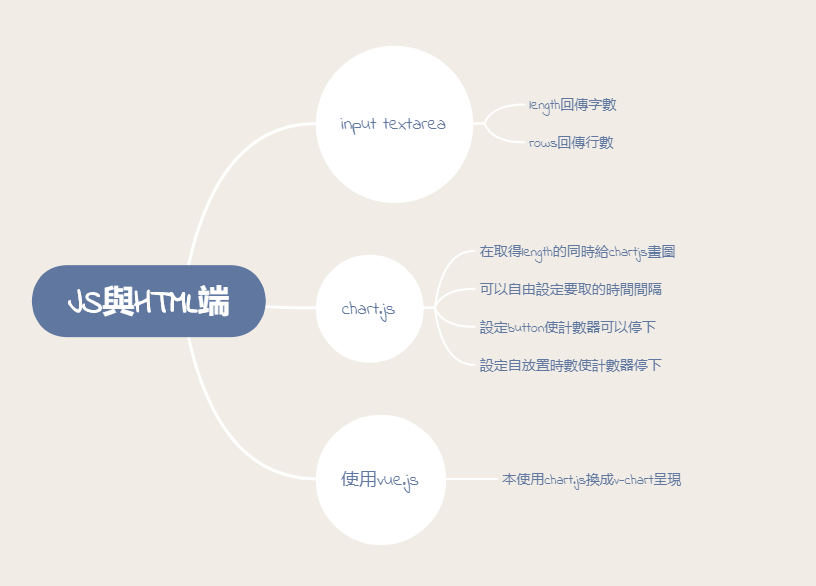
\includegraphics[width = .8\textwidth]{c5C4T4t.png}
\begin{figure}[H] %H为当前位置,!htb为忽略美学标准,htbp为浮动图形
		\centering %图片居中
		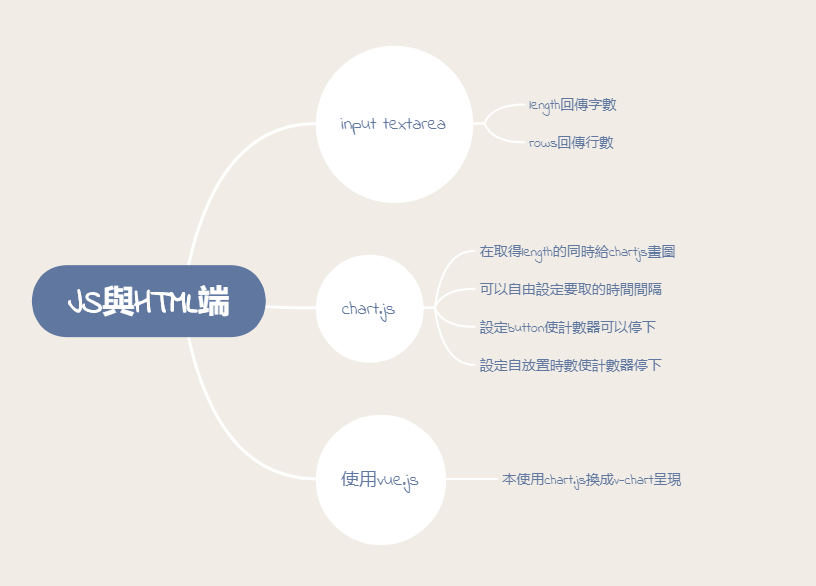
\includegraphics[width=0.7\textwidth]{1.png} %插入图片,[]中设置图片大小,{}中是图片文件名
		\caption{從JS、HTML以及Vue所打造的前端網頁中擷取資料} %最终文档中希望显示的图片标题
		\label{Fig.3.1} %用于文内引用的标签
\end{figure}
\subsection{模擬平台}
\begin{itemize}
	\item 目前所使用的解題平台雛形,其作答畫面如下圖所示。
	\begin{figure}[H]
		\centering
		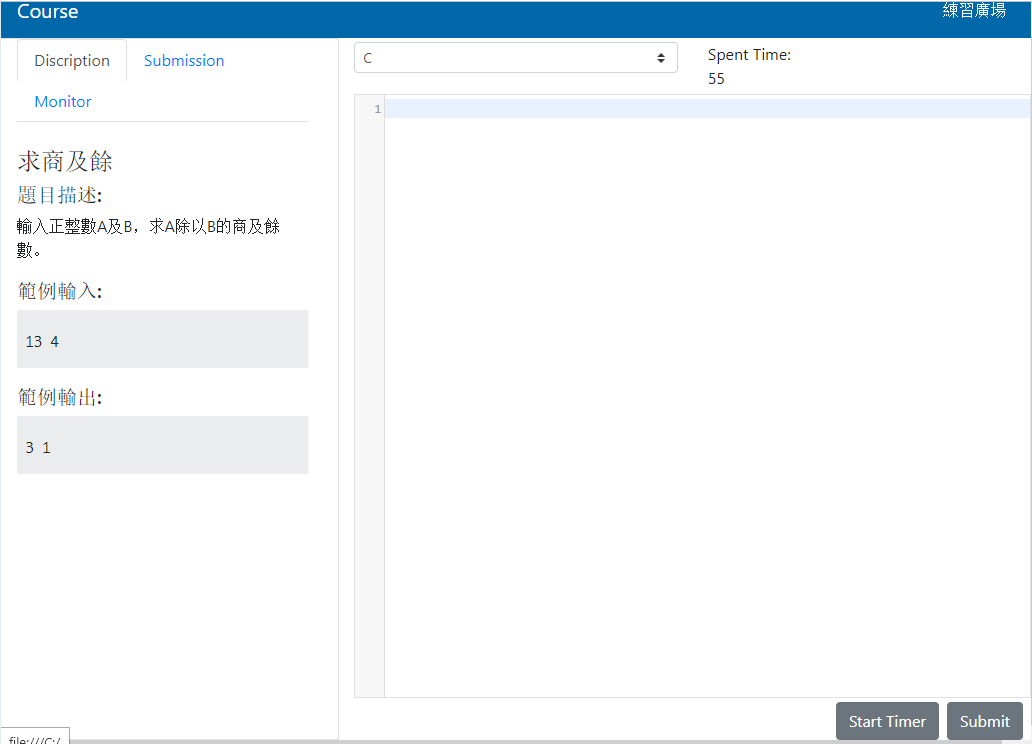
\includegraphics[width=0.7\textwidth]{web_part.png}
		\caption{模擬平台介面}
		\label{Fig.3.2}
	\end{figure}
	\item 功能:\\
	\begin{enumerate}[1.]
		\item 左方:顯示使用者正在作答的題目,包括輸入輸出的範例,供使用者了解目前作答的題目。使用者投稿之後,系統會自動切換至Submission頁籤,這個頁籤是評判伺服器進行評測之後所回傳的結果,包括答題正確狀況以及程式碼的格式檢查結果。
		\item 右上計算時間讀秒:右上的計時器記錄使用者所耗費的作答時間,每隔一定時間,系統會自動擷取使用者所輸入的內容,連同當時耗費的時間傳送到Firebase資料庫中。
		\item 右下的Stop Timer:暫停計時和傳送資料,目前做為除錯用途。
	\end{enumerate}
\end{itemize}

\subsection{基本統計資訊}
\begin{itemize}
	\item 字數與行數的判讀與計算\\
	取得使用者輸入的程式碼內容後,使用以下JS指令計算總共輸入的字數和行數:

\begin{lstlisting}[caption=js字數與行數的判讀與計算]
// code = 使用者輸入的程式碼內容
chars = code.length;
lines = 1+code.match(/\r?\n|\r/g).length; // 使用正規表達式尋找換行符號
\end{lstlisting}
此處用來判斷行數據的方法,主要是偵測使用者所用到的換行符號。如果使用者的程式碼文字中有其他的換行文字,可能會造成誤差。這個部份,未來可以使用鍵盤偵測來進行改良。計算出來的統計數字會使用HTML頁面顯示出來。

\item 時間的判讀與計算\\
目前用來擷取資料的方法主要是透過JS的setInterva函式,setInterval函式可以每隔一個設定時間不斷重覆執行特定的任務,在這裡主要是擷取使用者的作答內容。\cite{name20}
應該注意的一點,當作答結束之後,或者停止擷取資料之後,也要把setInterval所建立的程序清除掉,否則它會一直留在網頁中不斷執行,有可能會造成系統的問題。
擷取到的資料被傳送到Firebase中,可以用來做接下來的數據分析。
\end{itemize}
\subsection{輸出}
\begin{itemize}
	\item 即時監測圖:\\
	使用者的輸入內容和時間傳送到firebase的資料庫之後,會自動傳送收據更新的訊息到監控程式,監控程式的目的是顯示同學作答的一些統計資訊。
	目前數據的監測先選定一位同學為主,同學作答的時間,與輸入的字數和行數會使用圖形顯示出來。這邊使用了chart.js與vue.js來顯示前端的數據圖形。
	(圖3.3)
	\begin{figure}[H] %H为当前位置,!htb为忽略美学标准,htbp为浮动图形
		\centering %图片居中
		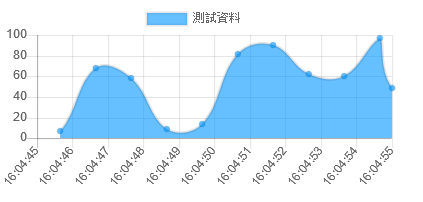
\includegraphics[width=0.7\textwidth]{3.png} %插入图片,[]中设置图片大小,{}中是图片文件名
		\caption{作答統計資訊範例} %最终文档中希望显示的图片标题
		\label{Fig.3.3} %用于文内引用的标签
	\end{figure}
呈現的統計圖每隔一段時間會隨著新的擷取資料而自動更新。資料擷取的時間間隔目前設定每秒一次,但可以隨著需要而做更改。圖表的 X 軸為時間,Y 軸為字數與行數。\\
	\item 影片輸出:\\
	除了進行數據監測及圖形繪製,另外也可以模擬同學作答過程的畫面,這部份一樣是Firebase傳送的數據更新資料,以畫面顯示當时同學的畫面,進行即時的監控。另外也可以根據這些資料,自動生成模擬同學作答畫面的影片,供教師或研究人員參考。
\end{itemize}
\section{基礎數據分析}
	\begin{figure}[H] %H为当前位置,!htb为忽略美学标准,htbp为浮动图形
	\centering %图片居中
	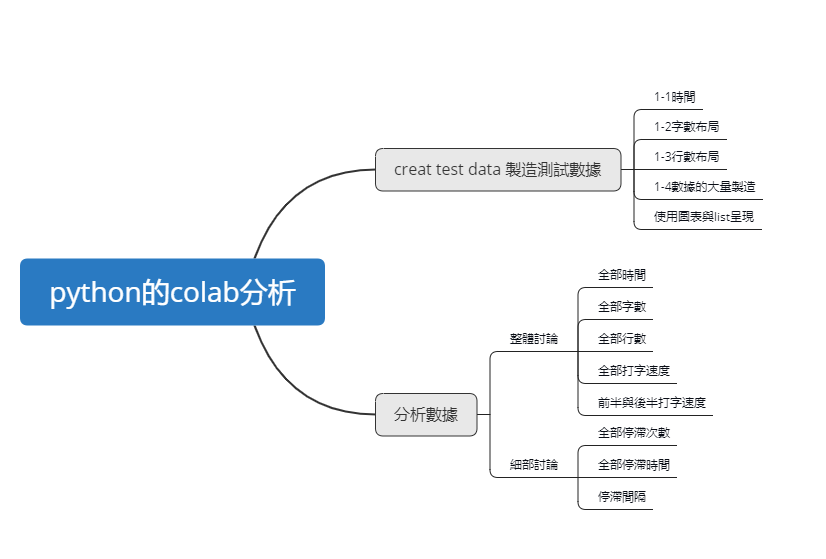
\includegraphics[width=0.7\textwidth]{2.png} %插入图片,[]中设置图片大小,{}中是图片文件名
	\caption{分析系統架構} %最终文档中希望显示的图片标题
	\label{Fig.3.4} %用于文内引用的标签
	\end{figure}
除了即時監測使用者的輸入狀況,我們也對收錄的資料做了一些基礎的統計分析,目前分析的內容包括:
1. 個別同學做一題的總時間分析,以及全部同學的平均作答時間
2. 停頓分析:如果作答的內容一直沒有改變,表示這位同學可能在某處卡住了。可以先找出停頓的位置,未來可以據此做更進一步的分析處理。

\subsection{模擬測試數據}
\subsubsection{討論數據的特徵}
圖(3.5)是典型作答過程的統計數字,因為是打字數與時間的關係,所以數據自然是漸進式的。圖中佔據面積比較大的部份為字數統計,下方面積比較小的部份為行數。
由於研究過程中,測試的作答平台尚未完整,因此除了採集一些個別少量的數據之外,先使用模擬產生的數據來進行分析,以觀察分析模組是否能正常運作。
	\begin{figure}[H] %H为当前位置,!htb为忽略美学标准,htbp为浮动图形
	\centering %图片居中
	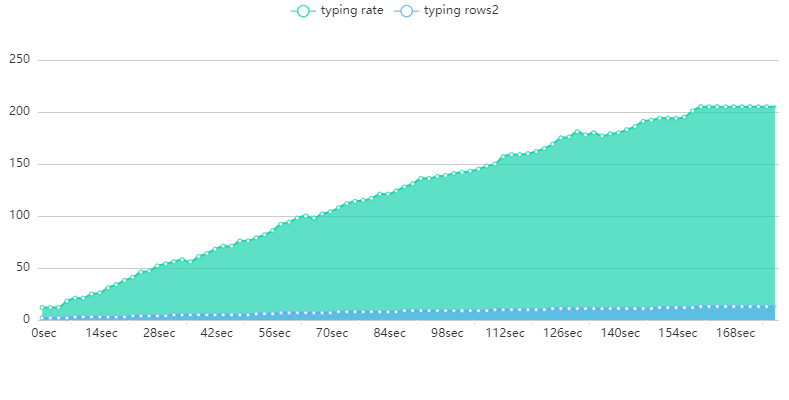
\includegraphics[width=0.7\textwidth]{4.png} %插入图片,[]中设置图片大小,{}中是图片文件名
	\caption{執行結果漸增圖} %最终文档中希望显示的图片标题
	\label{Fig.3.5} %用于文内引用的标签
	\end{figure}

在產生模擬數據之前,先討論一些作答數據的特徵和假設:
1. 規定時間區間:一個班級同學做同一題目,大家所完成的時間會有差別,可以規定自做的數據時間(ex:15分~1小時),而30分鐘可能是大部分人完成的時間,15分是做得快的,50分以上是做得慢的。
2. 作答字數:基本上整體分佈要像上圖一樣呈漸進增加的趨勢,但每位同學的字數增長速度可能不同,停頓的地方可能也不同,字數的增長也要設定一個合理的區間。
3. 作答行數:理論上越多字的越多行,但還是要在合理的範圍,不能生成太多行數。

\subsubsection{規定格式}
在統計圖(3.5)中包括三個欄位:時間、字數與行數。為了方便後續的分析,我們採用陣列的方式來儲存模擬數據。基本上模擬數據為三欄的陣列,其列數為模擬製造的記錄個數,以下分三部分說明各欄位數據的構成。
\subsubsection{時間欄位}
由於網頁程式擷取作答內容的時間間隔是固定的,因此為時間欄位為固定間隔的時間序列。(圖3.6)
	\begin{figure}[H] %H为当前位置,!htb为忽略美学标准,htbp为浮动图形
	\centering %图片居中
	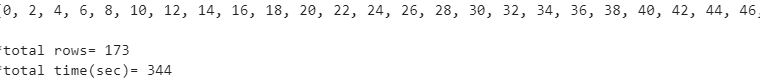
\includegraphics[width=0.7\textwidth]{3_2_1_3.png} %插入图片,[]中设置图片大小,{}中是图片文件名
	\caption{網頁程式執行結果圖} %最终文档中希望显示的图片标题
	\label{Fig.3.6} %用于文内引用的标签
	\end{figure}
每位同學在撰寫時所完成的時間也不相同,在產生數據時規定上下界,如同規定最快完成與最慢完成所需花費的時間。

\begin{lstlisting}[language=Python,caption=時間欄位的模擬數據]
data_up = 180
data_down = 500  #可以自行規定秒數區間
random_data = random.randint(data_up,data_down) #這是秒數
r1 = list(range(0,random_data,2)) #r1是第一部分時間陣列的部分
print(r1)
r_row1=len(r1)
r_row2=r1[-1]
print("\n*total rows=",r_row1,)
print("*total time(sec)=",r_row2) #計算random的格數與秒數(秒數為最後一個數據)
\end{lstlisting}
使用random函數進行最大秒數的選擇,後頭的第二與第三數據產生也大量地使用random函數。

\subsubsection{模擬字數}
這個部份可以說是最重要和最複雜的部份,因為使用者作答過程可能會有很多不同的變化。最初的構想的是使用者
作答的字數每次取樣都會不停地增加,但每次增加的字數不同,先使用亂數來模擬增加的字數。

\begin{lstlisting}[language=Python,caption=作答字數的模擬數據]
a = random.randint(0,10)
b = random.randint(a,20)
c = random.randint(b,30)
d = random.randint(c,40)
e = random.randint(d,50)
f = random.randint(e,60)
g = random.randint(f,70)
h = random.randint(g,80)
print(a,b,c,d,e,f,g,h)
\end{lstlisting}

如此,此程式所呈現的結果是(8 13 21 34 38 59 64 67),當然每執行一次都不同。
但這樣一來,使用者作答的字數會無止盡的增加,但這樣的方式沒有辦法反映使用者遇到不會的地方而卡住的情況,
所以要加入"使用者在思考"的停頓狀況,也就是會要維持同樣的字數一段時間。

除了停頓之外,使用者也有可能打錯字而按下倒退(Backspace)鍵,另外也可能使用了選擇和刪除的功能,
所以整體的數據並不會一路平滑的增加,必須在模擬數據中加上這些考量才比較合理。

於是我們新增三個模擬參數,分別用來處理增加、停頓、倒退和刪除的不同情況,
先使用random函數決定使用者可能的三個動作,而在增加與減少的時候,
數據的變化量是不均勻的,此部分一樣使用random函數來實現,如圖3.7所示。
\begin{figure}[H] %H为当前位置,!htb为忽略美学标准,htbp为浮动图形
	\centering %图片居中
	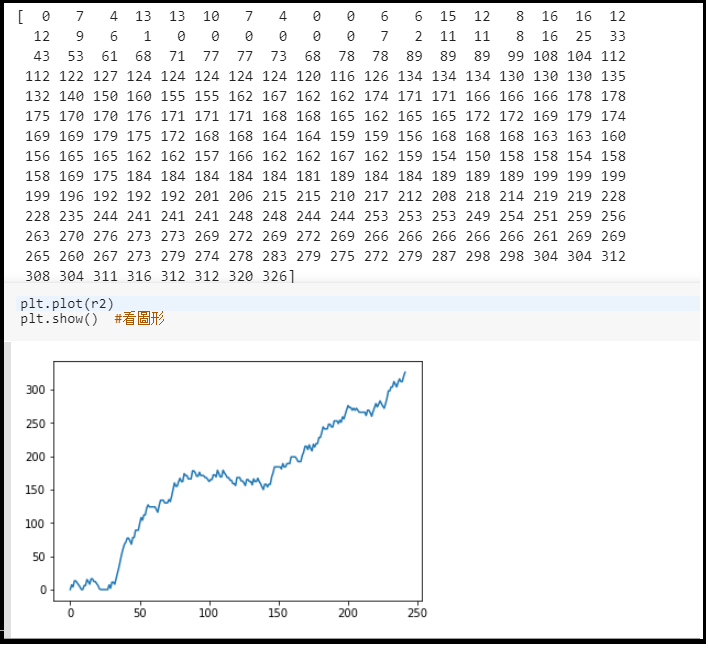
\includegraphics[width=0.7\textwidth]{3_2_1_4.png} %插入图片,[]中设置图片大小,{}中是图片文件名
	\caption{作答字數的模擬改良} %最终文档中希望显示的图片标题
	\label{Fig.3.7} %用于文内引用的标签
\end{figure}

\subsubsection{模擬行數}
第三部分為作答行數,這部分與字數息息相關,但是換行的判斷比較簡單,一般只要觀察原始程式碼是否有換行符號即可得知。此處是製
造出0,0,0,1,1,1,2,2,2,3,3,3,3,3,3,3,4,4,4,.....之類的漸增數列,但是增加的幅度遠比第二部分的字數還要緩慢許多。(圖3.8)
	\begin{figure}[H] %H为当前位置,!htb为忽略美学标准,htbp为浮动图形
	\centering %图片居中
	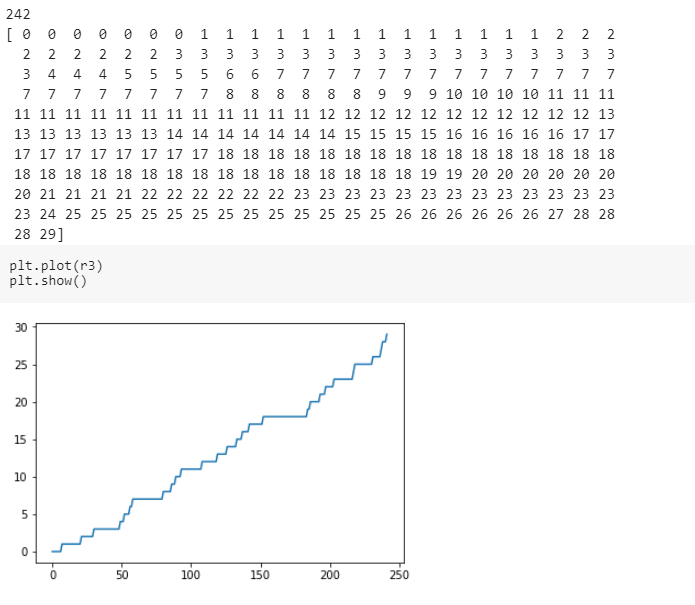
\includegraphics[width=0.7\textwidth]{3_2_1_5.png} %插入图片,[]中设置图片大小,{}中是图片文件名
	\caption{作答行數的數據模擬} %最终文档中希望显示的图片标题
	\label{Fig.3.8} %用于文内引用的标签
	\end{figure}

\subsection{數據分析}
\subsubsection{單組數據整體分析}
\begin{itemize}
	\item 可從最為直觀的記算所有數據的平均速度或是平均字數為基礎,在加上停頓點的分析。
	因為把數據設計成三欄的陣列,在分析步驟可以很容易抓到要的數據進行運算。
	\item 在陣列上最容易計算的如:作答時間、做答完畢字數、做答完畢(圖3.9)
	\begin{figure}[H] 
		\centering 
		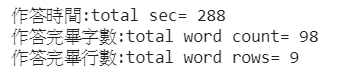
\includegraphics[width=0.7\textwidth]{3_8.png} 
		\caption{整體結果} 
		\label{Fig.3.9} 
	\end{figure}
	然後往下延伸計算的數據,如平均做答速度、前半作答速度、後半作答速度;在速度的計算上分兩部分是因為如果只有一個均速可能在比較上會有較大誤差,因此做多個速度的比較數據會更佳。(圖3.10)
	\begin{figure}[H] 
		\centering 
		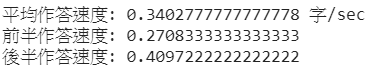
\includegraphics[width=0.2\textwidth]{3_9.png} 
		\caption{整體速度結果} 
		\label{Fig.3.10} 
	\end{figure}
	\item 收集這些速度的數據在之後比較多組,也就是多個同學更能知道每個人的打字速度,除了分析打字的字數外速度也可以加入進行細部分的分析。
\end{itemize}

\subsubsection{單組數據細部分析}
\begin{itemize}
	\item 除了單組數據的整體分析,最總體的數據與平均時間外,打字的停滯點也是至關重要。
	\item 要找出數組中的斷點若是直接觀察是非常容易的,如(圖3.10)
		\begin{figure}[H] 
		\centering 
		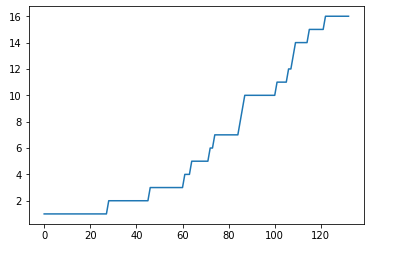
\includegraphics[width=0.7\textwidth]{3_10.png} 
		\caption{示例圖片} 
		\label{Fig.3.11} 
	\end{figure}
	若是看到打字沒有增加,在圖中是平行線段,就代表動作停滯、維持同一字數。
	\item 找出停滯部分本研究所使用方法是,使陣列的後項數據剪去前項數據,並且判斷此數據值若是正數,則判斷增加;若是0,判斷停滯;若是負數,判斷刪除倒退。
	可將此判斷數據化存成另一陣列,在此以下稱trend陣列。\\
	1. 後項減去前項為正:打字字數增加,1表示\\
	2. 後項減去前項為零:打字字數不變,0表示\\
	3. 後項減去前項為負:打字字數減少,-1表示\\
	將判斷後1,0,-1的值存入trend陣列,故此陣列為三個元素組成,且比原本數據的陣列值少一,因為trend陣列是原陣列間隔中的差分。(圖3.12)
		\begin{figure}[H] 
		\centering 
		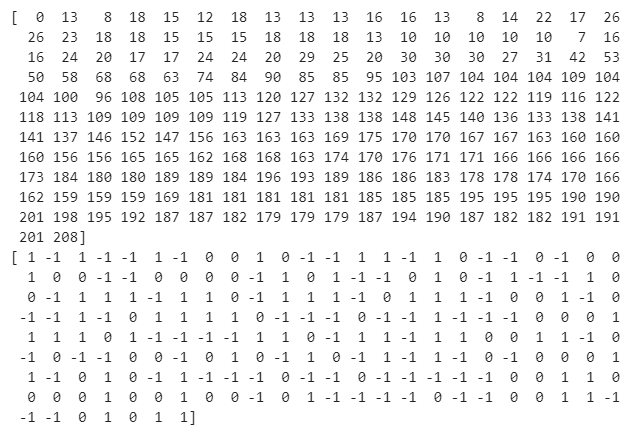
\includegraphics[width=0.7\textwidth]{3_11.png} 
		\caption{trend陣列輸出} 
		\label{Fig.3.12} 
	\end{figure}
	上半部陣列為原數據的陣列,字數遞增;下半部為使用1,0,-1判斷產生的trend陣列。
	如此便很清楚的看出,0是使用者停下的部分,之後能從0所停頓的時間長度,或是停頓所發生的次數判斷分析。
	\item 除了把trend陣列顯示外,若能畫圖更能掌握此陣列數據的特徵。(圖)點狀圖
	\begin{figure}[H] 
		\centering 
		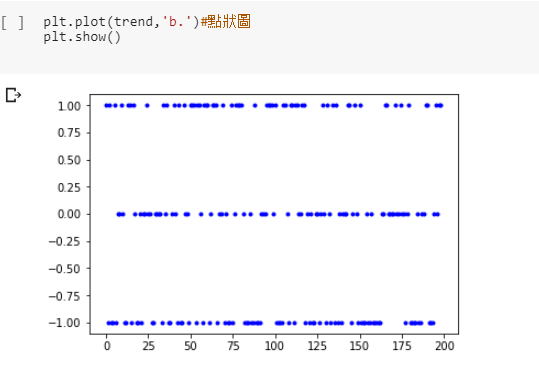
\includegraphics[width=0.7\textwidth]{3_12.png} 
		\caption{trend點狀圖} 
		\label{Fig.3.13} 
	\end{figure}
	(圖)圓餅圖
	\begin{figure}[H] 
		\centering 
		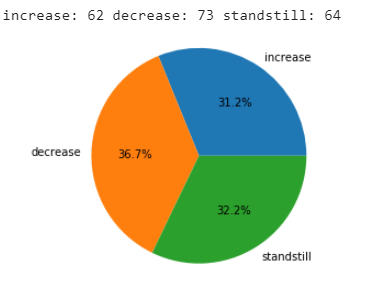
\includegraphics[width=0.7\textwidth]{3_13.png} 
		\caption{trend圓餅圖} 
		\label{Fig.3.14} 
	\end{figure}
\item 製做點狀圖或是圓餅圖可以顯示使用者停頓、打字或是刪除的密集程度。不過此處若是希望只看停頓處的地方,於是在多新增一個新的陣列,以下稱trend2。trend2是把0的元素抓出,把0換成1;因此trend2數據便只有0與1數值。
\item 部分程式:
\begin{lstlisting}[language=Python,caption=python數據trend2]
#len(trend)#trend的隔數 大約表示時間的1/2
trend2=np.zeros(len(trend),int)
for j in range (0,len(trend2)):
	if (trend[j]!=0):
		trend2[j]=0
	else :
		trend2[j]=1
print(trend)
print(trend2)#trend2是trend的停頓部分
\end{lstlisting}
將trend與trend2顯示(圖3.15)
	\begin{figure}[H] 
	\centering 
	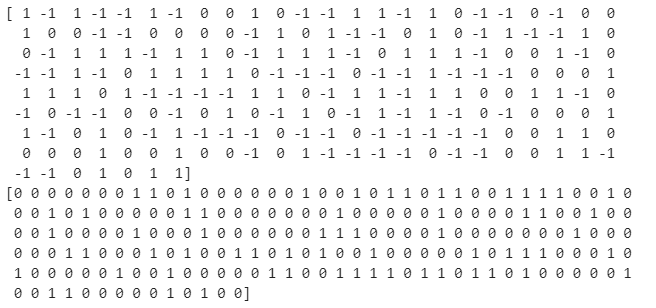
\includegraphics[width=0.7\textwidth]{3_14.png} 
	\caption{trend2輸出} 
	\label{Fig.3.15} 
\end{figure}
\newpage
如此只剩0與1兩個元素的trend2陣列畫成柱狀圖觀察,如同條碼的形狀。(圖3.16)其中線條就是使用者停頓處。
	\begin{figure}[H] 
	\centering 
	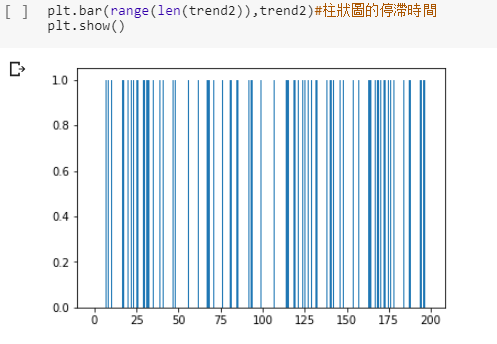
\includegraphics[width=0.7\textwidth]{3_15.png} 
	\caption{trend2條碼狀方圖} 
	\label{Fig.3.16} 
\end{figure}
\item 最後一個圖做分區的統計,這裡計算trend2陣列1的出現次數,並且做分區的統計次數。
分區的分法是察看trend2的全部元素個數,並且分成五等分,在一個個部分統計停頓的出現次數,例如若有200數據,則第一部份統計1出現個數為0~50組,第二部分統計為50~100,以下類推。(圖3.17)
	\begin{figure}[H] 
	\centering 
	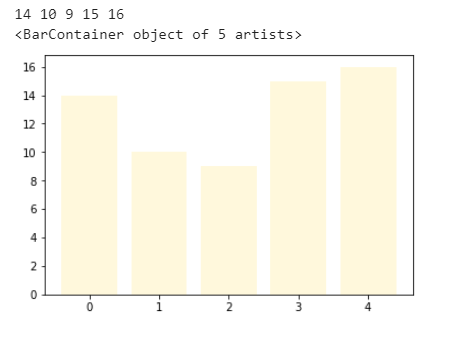
\includegraphics[width=0.7\textwidth]{3_16.png} 
	\caption{trend2分區圖} 
	\label{Fig.3.17} 
\end{figure}
不過如此計算的密度為強制分區,可能無法把密度情況很好的呈現出來,此部份討論於結果部份做詳細討論檢討。
\end{itemize}
\subsubsection{多組數據}
以上分析都是只使用一組數據分析與統計的結果,若要在此基礎上擴增成多數據的分析,則需要進行更多數據的製造與集合分析,所以以上的步驟需要進行多次。
如此進行多次迴圈,此迴全次數可以自行修改。(圖3.18)為設定10次所呈現之全部格數與全部時間。
\begin{figure}[H] 
	\centering 
	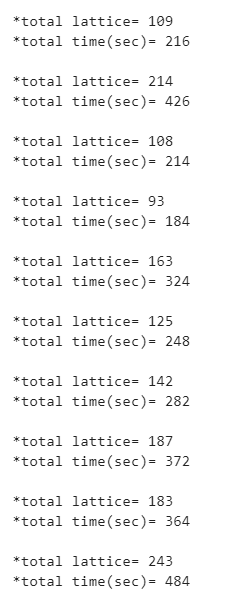
\includegraphics[width=0.5\textwidth]{3_17.png} 
	\caption{多組數據} 
	\label{Fig.3.18} 
\end{figure}


\chapter{實驗與執行結果}
%\label{c:intro}
本章節討論網頁與分析的結果與輸出數據
\section{網頁平台數據結果}
\subsubsection{顯示頁面}
在網頁的平台只有觀察使用者打字與紀錄時間並畫圖顯示。(圖4.11)為網頁偵測的頁面,有一空白處就是給使用者打字的地方,並且在進行打字同時計算字術語時間回傳,進而畫出時間字數的折線圖。
	\begin{figure}[H] 
	\centering 
	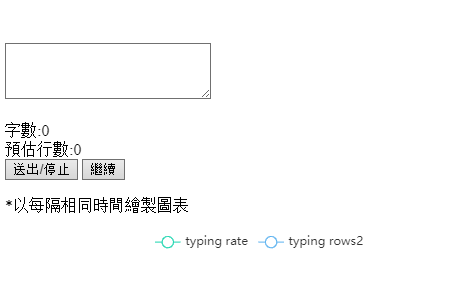
\includegraphics[width=0.7\textwidth]{4_1.png} 
	\caption{網頁顯示頁面} 
	\label{Fig.4.1} 
	\end{figure}
\subsubsection{網頁的圖形輸出}
因本研究是基於討論學生在做題目的分析,於是我找了一些文字試打並擷取回傳的圖形畫面結果:
\begin{enumerate}[1.]
	\item 簡短程式碼(圖4.2)
	\begin{figure}[H] 
		\centering 
		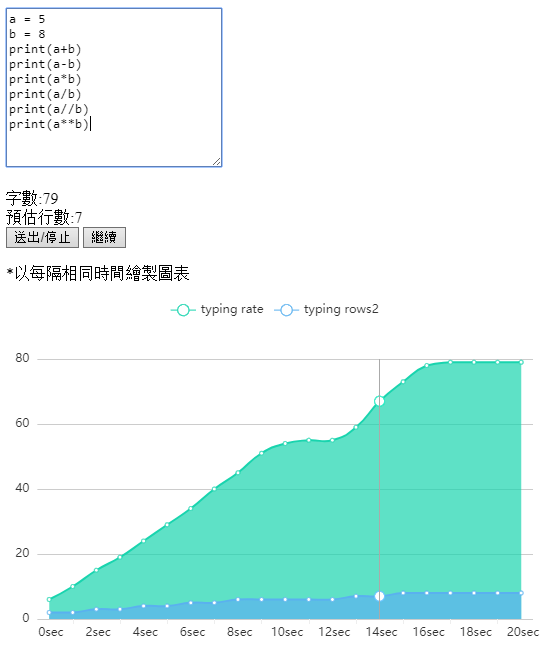
\includegraphics[width=0.7\textwidth]{4_2.png} 
		\caption{簡短程式碼輸出} 
		\label{Fig.4.2} 
	\end{figure}
	\item 簡短中文字(圖4.3)\\
	在打中文字時我所打錯的地方較多,所以使用backspace倒退鍵的情況也變多了,所以圖上呈現才會有更多的彎曲;上升一點下降一點就是使用者在改錯的地方。
	\begin{figure}[H] 
		\centering 
		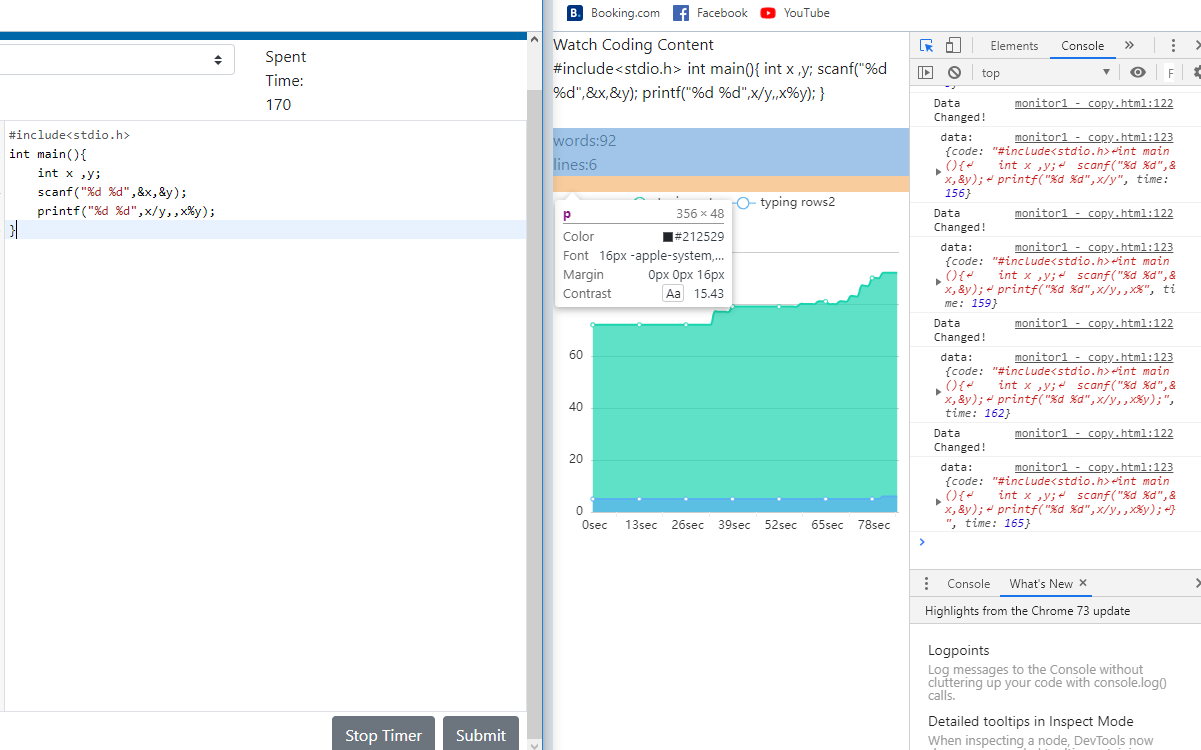
\includegraphics[width=0.7\textwidth]{4_3.png} 
		\caption{簡短中文字輸出} 
		\label{Fig.4.3} 
	\end{figure}
	\item 複製貼上(圖4.4)\\
	若是使用者貼上大量文字的話,圖形變化會成階梯狀因數據變化的幅度比自行打字大很多,因此如使用者使用了貼上鍵,此頁面是能夠偵測到的。
	\begin{figure}[H] 
		\centering 
		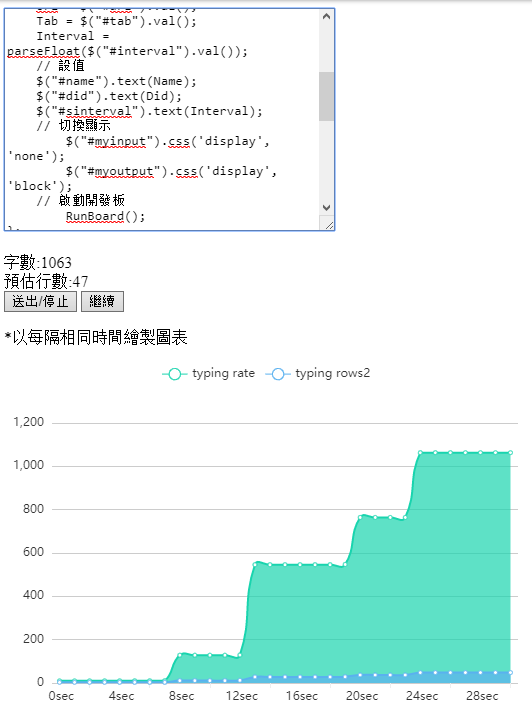
\includegraphics[width=0.7\textwidth]{4_4.png} 
		\caption{複製貼上輸出} 
		\label{Fig.4.4} 
	\end{figure}
\end{enumerate}
\section{python的討論分析}
因本研究所寫的python程式碼可以指定實驗數據的數量進進行製作與分析,在此便指定10組與30組結果。
\subsubsection{個別的圖形與數據}
每一組數據便會產生(圖4.5)的一組圖形,在此便不把全部圖形列出,以下只列每次產生的數據最基本的折線圖,共10組。(圖4.6)
	\begin{figure}[H] 
	\centering 
	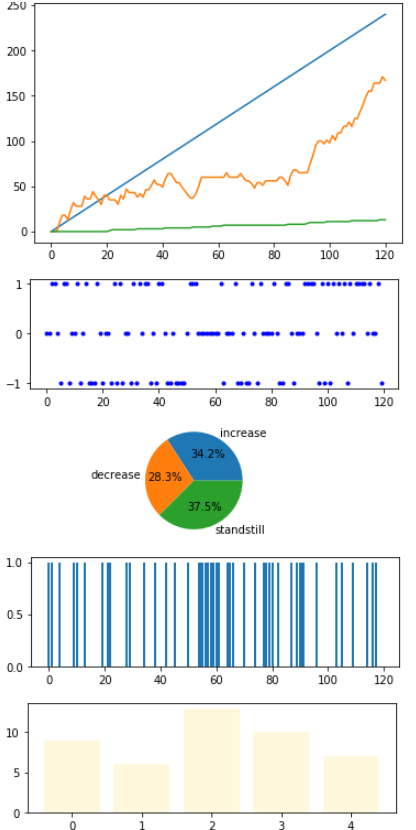
\includegraphics[width=0.7\textwidth]{4_5.png} 
	\caption{圖形組} 
	\label{Fig.4.5} 
	\end{figure}
	\begin{figure}[H] 
	\centering 
	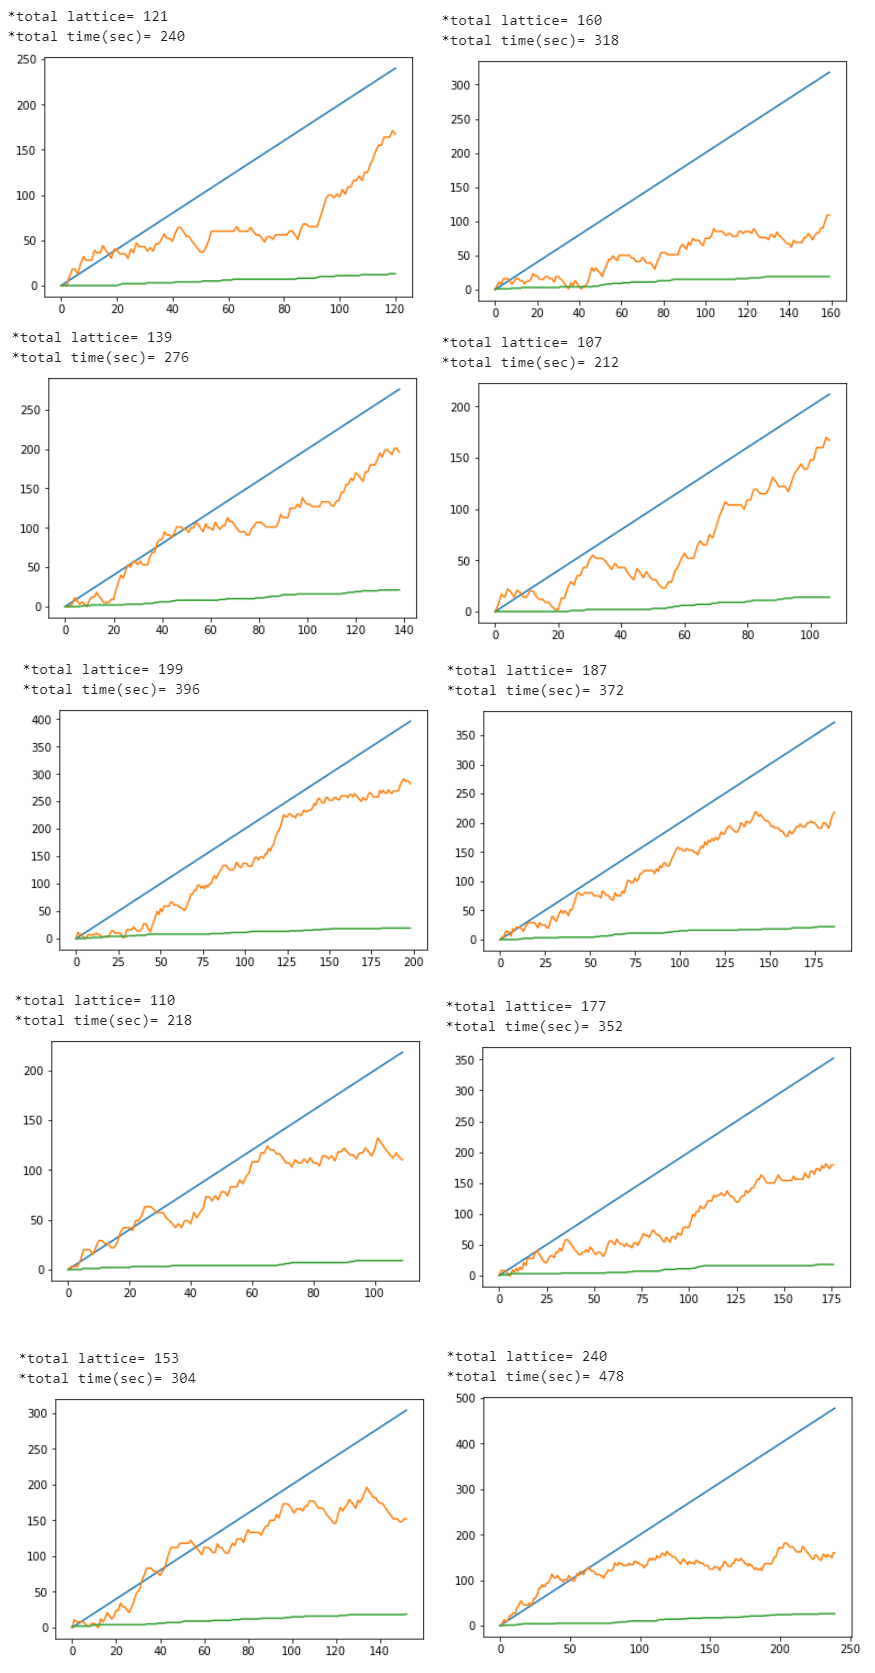
\includegraphics[width=0.7\textwidth]{4_6.png} 
	\caption{10組折線圖} 
	\label{Fig.4.6} 
	\end{figure}
\subsubsection{統整的表格數據}
把全部的數據統整起來製程表格,表格也是使用python在colab可以輸出顯示結果。\\
1. 10組結果(圖4.7)
	\begin{figure}[H] 
	\centering 
	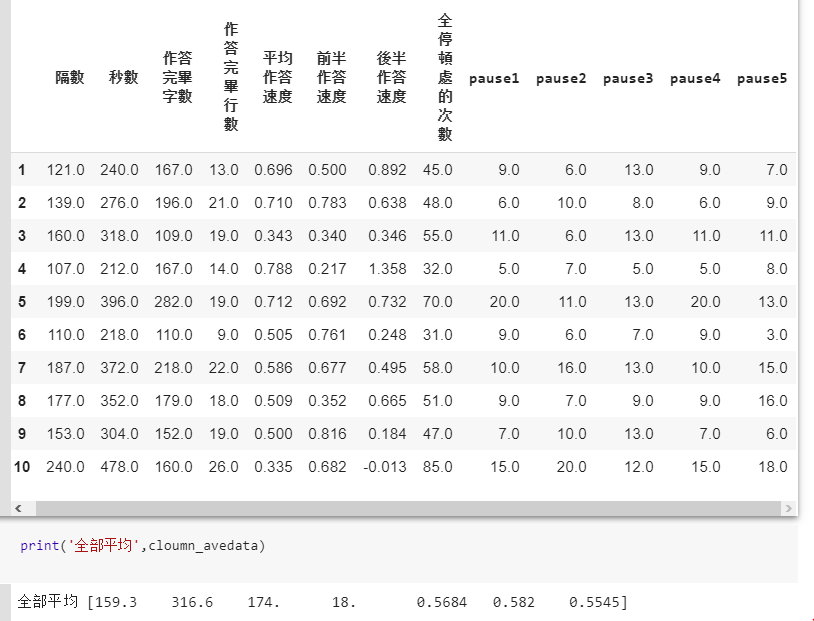
\includegraphics[width=0.7\textwidth]{4_7.png} 
	\caption{10組結果表格圖} 
	\label{Fig.4.7} 
	\end{figure}
\newpage
2. 30組結果,因資料較龐大所以使用表格顯示(表4.1))\\
\begin{table}[]
	\label{table1}
	\begin{tabular}{lllllllll}
		& 隔數  & 秒數  & 作答完畢字數 & 作答完畢行數 & 平均作答速度 & 前半作答速度 & 後半作答速度 & 全停頓處的次數 \\
		1  & 115 & 228 & 193    & 19     & 0.846  & 0.833  & 0.86   & 39      \\
		2  & 190 & 378 & 343    & 14     & 0.907  & 0.984  & 0.831  & 72      \\
		3  & 212 & 422 & 230    & 26     & 0.545  & 0.417  & 0.673  & 69      \\
		4  & 149 & 296 & 204    & 12     & 0.689  & 0.716  & 0.662  & 52      \\
		5  & 172 & 342 & 246    & 17     & 0.719  & 0.374  & 1.064  & 53      \\
		6  & 135 & 268 & 94     & 15     & 0.351  & 0.425  & 0.276  & 46      \\
		7  & 219 & 436 & 299    & 26     & 0.686  & 0.583  & 0.789  & 67      \\
		8  & 133 & 264 & 189    & 19     & 0.716  & 0.803  & 0.629  & 51      \\
		9  & 111 & 220 & 171    & 11     & 0.777  & 1.509  & 0.045  & 31      \\
		10 & 127 & 252 & 80     & 15     & 0.317  & 0.516  & 0.119  & 47      \\
		11 & 140 & 278 & 242    & 19     & 0.871  & 0.964  & 0.777  & 51      \\
		12 & 241 & 480 & 288    & 26     & 0.6    & 0.354  & 0.846  & 77      \\
		13 & 222 & 442 & 371    & 25     & 0.839  & 1.009  & 0.67   & 70      \\
		14 & 220 & 438 & 288    & 28     & 0.658  & 0.749  & 0.566  & 71      \\
		15 & 247 & 492 & 218    & 28     & 0.443  & 0.472  & 0.415  & 84      \\
		16 & 158 & 314 & 176    & 18     & 0.561  & 0.924  & 0.197  & 52      \\
		17 & 162 & 322 & 136    & 17     & 0.422  & 0.472  & 0.373  & 61      \\
		18 & 227 & 452 & 267    & 29     & 0.591  & 0.633  & 0.549  & 81      \\
		19 & 199 & 396 & 139    & 19     & 0.351  & 0.641  & 0.061  & 75      \\
		20 & 240 & 478 & 209    & 32     & 0.437  & 0.552  & 0.322  & 75      \\
		21 & 202 & 402 & 178    & 25     & 0.443  & 0.597  & 0.289  & 61      \\
		22 & 189 & 376 & 349    & 22     & 0.928  & 0.793  & 1.064  & 53      \\
		23 & 203 & 404 & 161    & 26     & 0.399  & 0.302  & 0.495  & 65      \\
		24 & 146 & 290 & 197    & 8      & 0.679  & 1.186  & 0.172  & 48      \\
		25 & 195 & 388 & 185    & 17     & 0.477  & 0.629  & 0.325  & 70      \\
		26 & 93  & 184 & 61     & 10     & 0.332  & 0.946  & -0.283 & 25      \\
		27 & 98  & 194 & 60     & 2      & 0.309  & 0.33   & 0.289  & 28      \\
		28 & 93  & 184 & 132    & 8      & 0.717  & 0.772  & 0.663  & 33      \\
		29 & 204 & 406 & 225    & 18     & 0.554  & 0.951  & 0.158  & 65      \\
		30 & 120 & 238 & 91     & 16     & 0.382  & 0      & 0.765  & 52     
	\end{tabular}
\caption{30組數據}
\end{table}
\newpage
\section{結果討論}
\subsection{html網頁偵測部份}
\begin{itemize}
	\item 本研究藉由網頁前端及時偵測使用者的打字情況,並且計算其字數與花費時間。不同於其餘答題系統需要繳交後才知曉使用者的答題狀況,此方法因為其實時偵測的特性,使用者的答題習慣也可以藉由字數與時間看出端倪。
	\item 在網頁上只擷取了字數、行數與時間,如可以增加更多的鍵盤偵測將會使系統更加完善,此處為能多加以改良完善的地方。
\end{itemize}
\subsection{python分析部分討論}
\begin{itemize}
	\item 進行分析的部分最大的難處就是缺少實際數據,因此在本文中使用程式去模擬實際的數據。但是因在此使用大量的radom函數與諸多限制,如為了使程式撰寫方便設的上下界線使數據密集化等。模擬的數據理所當然地不及實際數據來的真實與客觀。
	\item 再討論數據停頓的密集程度的地方(圖3.16),我所選用的方法是把整體數據分成五個等分並寫計算每一等分的停頓次數;而此部分也是不夠嚴謹的,因可能密集的地方會被分組計算而分割,所以分區計算的方法並不能表示絕對的疏密程度。
\end{itemize}
\chapter{結果討論與未來展望}
%\label{c:intro}
本論文主要針對線上解題平台,製作了一個即時監控與數據分析的子系統。目前可以在作答的雛形平台上進行資料的採集,自動上傳到Firebase的雲端資料庫中,
並且可以自動產出一些基本的作答統計資料和圖形。另外也可以透過擷取的資料,產出模擬作答的畫面和影片檔,以及進行一些基礎的資料分析。\\
本研究所提出的方法還有很多可以改進的空間,例如在偵測與製作影片檔因有擷取數據的間隔,會產生延遲較大的現象;亦或因為缺少大量實際數據而使用模擬數據進行分析等等。未來可以根據這些基礎繼續擴充及改良,希望可以更加完善,並可以成為未來更具人工智能的作答平台的一個基礎。

%\input{conclusion}

\appendix

\backmatter

\addcontentsline{toc}{chapter}{\bibname}
\bibliographystyle{unsrt}

% Your bibliography goes here
\bibliography{thesis}
%\bibliography{references}{}
%\bibliographystyle{unsrt}
\end{document}
